\documentclass[12pt, a4paper]{report}
\usepackage{amsmath}
\usepackage{graphicx}

\title{Assignment 1 \\
}
%\subtitle{Part A}

\author{Rahul Wankhede}
%\date{September 8, 2019}

\begin{document}

\maketitle

\begin{center}
\section*{Part A}
\end{center}

\subsection*{c) Load}
\subsubsection*{Array}

Space Complexity Analysis: \\
For Array, space taken should be O($n^2$) \\
For CSR, space taken = O(NNZ) \\~\\
Time Complexity Analysis: \\
Array = O($n^2$) \\
CSR = O(NNZ) \\~\\
Experimental Observations: \\

%Array size (nxn) vs Load Array times (in milliseconds)
\begin{center}
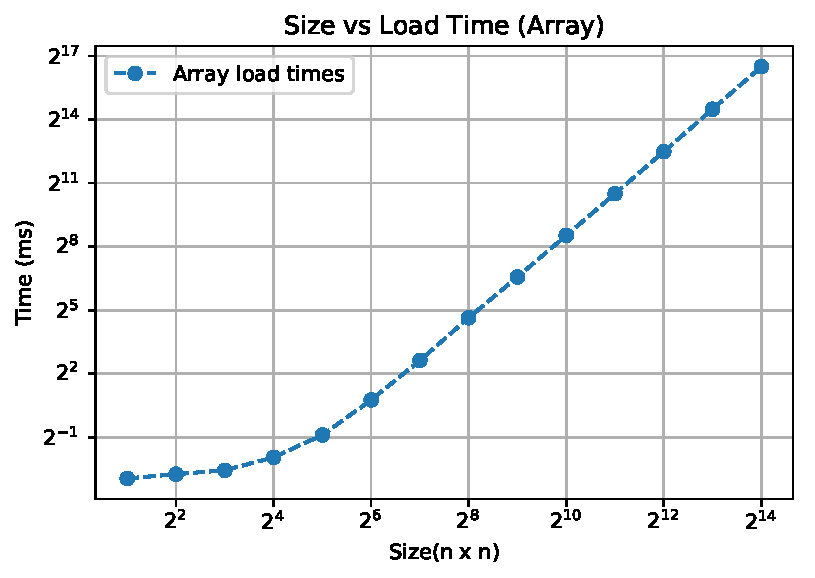
\includegraphics{load_arr.pdf}
\end{center}


\subsubsection*{CSR}
Due to some error, that I don't know yet how to solve, I couldn't load any CSR that is of size 8x8 or greater.
The exact error encountered is: \\~\\
\textit{*** stack smashing detected ***: ./Runner.o terminated \\
Aborted}


\subsection*{d) Transpose}
Space Complexity Analysis: \\
For Array, space = O($n^2$) \\
For CSR, space taken = O(NNZ) \\~\\
Time Complexity Analysis: \\
Array = O($n^2$) \\
CSR = O(NNZ) \\~\\
Experimental Observations: \\

\begin{center}
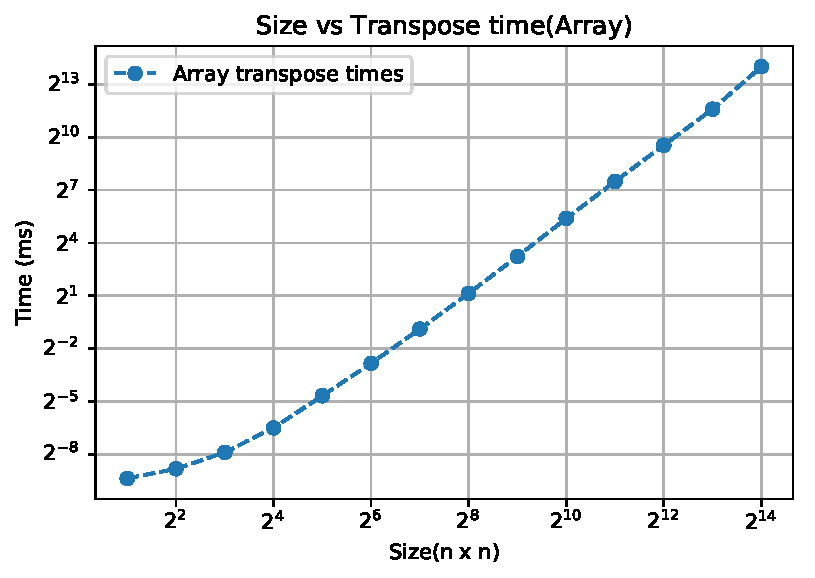
\includegraphics{transpose_arr.pdf}
\end{center}



\newpage

\subsection*{e) Multiply}
Space Complexity Analysis: \\
For Array, space = O($n^2$) \\
For CSR, space taken = O(NNZ) \\~\\
Time Complexity Analysis: \\
Array = O($n^3$) \\
CSR = O(NNZ) \\~\\
Experimental Observations: \\

\begin{center}
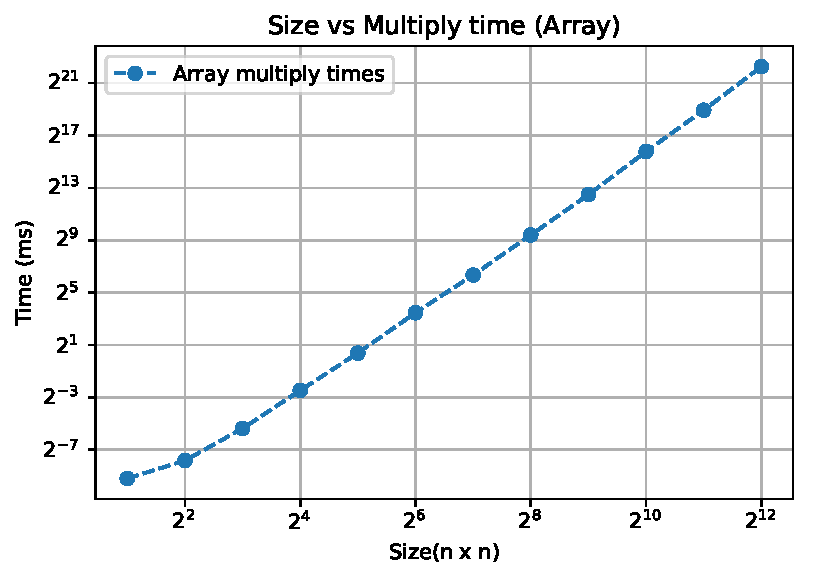
\includegraphics{multiply_arr.pdf}
\end{center}


\newpage


\begin{center}
\section*{Part B}
\end{center}


\end{document}

